%        File: learnability.tex
%     Created: Mon Feb 06 11:00 AM 2017 E
% Last Change: Mon Feb 06 11:00 AM 2017 E
%
% arara: pdflatex: {options: "-draftmode"}
% arara: biber
% arara: pdflatex: {options: "-draftmode"}
% arara: pdflatex: {options: "-file-line-error-style"}
\documentclass[MilwayThesis]{subfiles}

\begin{document}
In this section, I will evaluate some previous analyses of resultatives, based on their learnability, largely setting aside questions of over-/under-generation.
This choice of evaluation metric is motivated by the overall goals of this thesis and by the fact that questions of generative capacity are well-addressed by the analyses that I will evaluate.

The resultative parameter presents an acquisition problem for two broad reasons.
The first problem is that, on the surface, resultatives, which are parameterized, are indistinguishable from depictives, which appear to be universal.
The two construction types are indistinguishable in the sense that both correspond to the string template in \Next (modulo independent word order variation).
\ex. \textsc{Subj} V \textsc{Obj} Adj.

This indistinguishability is evident in the fact that one can construct examples which are truly ambiguous between resultative and depictive readings, as in \Next.
\ex. 
\a. He fried the fish dry.
\a. $\approx$ He fried the fish once it was dry. (\textbf{Depictive})
\b. $\approx$ He fried the fish until it was dry. (\textbf{Resultative})
\z.
\b. She painted the barn red.
\a. $\approx$ The barn is red in her painting. (\textbf{Depictive})
\b. $\approx$ She applied a coat of red paint to the door. (\textbf{Resultative})
\z.

Assuming a child acquiring either French or English encounters sentences with the form of \LLast in their PLD, there is no obvious way for the child to determine whether a given secondary predicate is to be interpreted depictively or resultatively.
<++>

The second problem is that <++>

One approach to the resultative parameter is what I will call the lexicalization account.
Under this account, event descriptions are decomposable into several universal features (\textit{e.g.}, \textsc{Result}, \textsc{Manner}, \textsc{Process}), and language variation results from languages lexicalizing these features differently.
One such an account by \textcite{son2008microparameters} proposes that English and German lexicalize \textsc{Result} in null heads, while Romance languages only lexicalize \textsc{Result} in verbs.
\ex.
\raisebox{-.9\height}{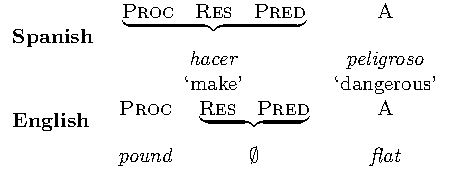
\includegraphics{lexicalization_table}}

\end{document}


